\input{/Users/joshyv/Research/misc/latex_paper.tex}
\usepackage{algorithmic}
\usepackage{algorithm}

\newtheorem{goal}{Goal}
\newtheorem{desid}{Desiderata}
\newcommand{\zz}{\mathbb{Z}}
\newcommand{\nec}{NeCoG}

\lhead{Vogelstein JT, et al}
\rhead{Neurocognitive Graph Theory}

\title{A Neurocognitive Graph Theoretical Approach to Understanding the Relationship Between Minds and Brains}

\author{Joshua T. Vogelstein, R. Jacob Vogelstein, Carey Priebe\\{Johns Hopkins University}}

\begin{document}

\maketitle

\paragraph{Current Paradigm}

The dominant paradigm of quantitative neuroscience in the 20$^{th}$ century has been the ``signal processing'' framework \cite{}.  Essentially, the brain is a box, that filters some stimulus, to produce some response (see Figure 1). This framework leads to the following goal:

\begin{goal}
	Learn the filter that the brain performs on stimuli to result in the actualized responses.
\end{goal}

\begin{figure}[h!]
\centering 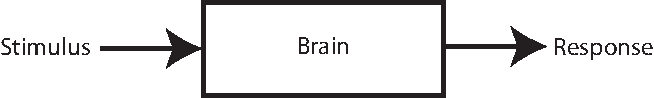
\includegraphics{stim_brain_resp}
\caption{The signal-processing paradigm of quantitative neuroscience.  The brain is a box that essentially \emph{filters} the stimulus, outputting some response, which is often take to be multivariate time series (such as populations of spike trains or fMRI activity).} \label{fig:SBR}
\end{figure}


This paradigm has been appropriate, given the kind of data available to people investigating the brain.  More specifically, the kind of data that has been most available has been time-series of signals related to neural activity \cite{}.  Given that electrical engineers were largely the individuals obtaining and analyzing the data, it was natural to take a signal-processing approach.  Often, the dynamic time-series data were used to estimate static parameters.  In the previous decades, these communities have been more and more sophisticated models and algorithms to estimate these parameters \cite{}.  Recently, issues such as parameter identifiability, consistency, bias, and model selection have been gaining traction as important desiderata for our models \cite{}.  

\paragraph{Alternate Paradigm}

Here, we define a different goal, which suggests a complementary research paradigm to the current dogma: %which we believe has not been satisfied by any previously proposed research paradigm.  Further, we elaborate on a novel paradigm that we believe is sufficient to satisfy this goal.

\begin{goal}
	Construct a family of brain-models, $\mB$, that is sufficient to provide \emph{causal} explanations relating properties of minds with properties of brains.
\end{goal}

Note how the above goal is distinct in certain respects from the ``filtering'' goal.  First, neither stimulus nor response is explicitly incorporated into this goal.  While stimuli and response may be used as tools to obtain the parameters of $\mB$, that is their only merit in this paradigm.  Second, minds are explicitly incorporated into this goal.  While spike trains or fMRI signal may indicate mental processes, they are likely not what is meant by ``mind''; rather, they may be used as tools to infer mental states.  Third, the inclusion of a class of models $\mB$  suggests a statistical \emph{static} framework, rather than a dynamics perspective.  In addition to the above stated goal, we would like the family of models $\mP$ to satisfy a number of desiderata:

\begin{enumerate}
	\item $\mB$ %$=\{\mathbb{P}_{\bth}; \bth \in \bTh\}$ 
	should be sufficiently general to account for whatever properties of the brain are casually related to the properties of cognition under investigation.
	\item The properties of any particular brain, $b\in \mB$, should be either measurable or estimatable, such that experimental observation may be used to obtain them.
	% \item Parameter estimates should be consistent \cite{} %, that is, $\hbth_n \conv \bth$ as $n \conv \infty$.
	\item $\mB$ should admit algorithms that (are guaranteed to be able to) capture the relationship of interest.
	\item $\mB$ should also admit \emph{causal} studies, which entail modifying a particular $b \in \mB$, to modify the corresponding mental property, $m \in \mM$.
\end{enumerate}


\paragraph{NeuroCognitive Graph Theory}

Here, we propose a novel approach, called NeuroCognitive Graph (NeCoG) theory, which we believe achieves the above goal and its associated desiderata.  Specifically, we say that the brain may be well characterized as a labeled, attributed multigraph (which is a generalized notion of a or network\footnote{I think binary graphs should probably go here, with extensions later.}).  Formally, we define a brain-graph, $b\in \mB$ as a 4-tuple, $\mB=(\mV,\mE,\mX_V, \mX_E)$, where

\begin{itemize}
	\item $V_i \in \mV \subseteq \mathbb{Z}$ for $i \in [V]$, is the set of vertices (nodes), where $[V]=\{1,2,\ldots,V\}$ 
	\item $E_{ijk} \in \mE \subseteq [V] \times [V] \times \mathbb{Z}$ for $(i,j,k) \in [V] \times [V] \times \mathbb{Z}$ is the set of (directed) edges, where $\zz=\{0,1,\ldots\}$
	\item $\bX_i \in \mX_V \subseteq \Real^{d_V}$ for $i \in [V]$ is the set of vertex attributes, and $d$ is the dimensionality of the vertex attributes (potentially including vertex labels)
	\item $\bX_{ijk} \in \mX_E \subseteq \Real^{d_E}$ for $(i,j,k) \in [V] \times [V] \times \zz$ is the set of edge attributes, $d'$ is the dimensionality of the edge attributes (potentially including edge labels), and $k$ indexes edge categories.
\end{itemize}


Assume, for the moment, that we take the fundamental computational unit of the brain to be a point neuron.  Then, each vertex is a neuron, and each edge is a synapse.   Multi-edges potentially correspond to different edge magnitudes and/or categorically different edges (like chemical and electrical synapses). Vertex attributes could include neurotransmitter released, proteins expressed, morphological properties, receptive fields, etc.  Edge attributes could include probability of release, post-synaptic potential shape, etc.  This level of description, however, is not necessary.  For instance, $\mV$ might instead correspond to neuroanatomical regions, which admit very different notions for edges and attributes.  This multi-scale aspect of $\mB$ is an important advantage over other frameworks.  

Given $\mB$, what can we do with it?  As stated above, our goal is to relate these models to properties of cognition. More specifically, let $\mM$ characterize the space of the cognitive (mental) property, and $g \in \mG$ be some function to learn.  

\begin{itemize}
	\item If $\mM=\{0,1\}$, then $g$ is a two-way classifier: $g: \mB \conv \{0,1\}$.
	\item If $\mM=\{0,1,\ldots, C\}$, then $g$ is an $C-$way classifier: $g: \mB \conv \{0,1,\ldots,C\}$.
	\item If $\mM=\Real^a$, then $g$ is a (multivariate-) regressor: $g: \mB \conv \Real^a$.  
\end{itemize}

In general, solving the above problems---which means finding $g$---will depend on $F=F_{BM}$, the joint distribution of brains and minds.  In practice, however, $F$ is unknown, and therefore $g$ must be estimated from the data. Assume we have a corpus of training data, $\mD_n=\{(B_1,M_1), \ldots, (B_n, M_n)\}$, where $n$ is the number of training samples.  Our goal then is to compute $g_n: \mB \times (\mB, \mM)^n \conv \mM$, which takes as input an observed brain-graph $b$ and $n$ training paris $\{(b_1,m_1), \ldots, (b_n,m_n)\}$ and produces a prediction $\hm=g_n(b; \mD_n)$.  The goal is to find a $g_n$ that minimizes some loss function, $L_F(g_n)$.  For instance, when $|\mM|=2$, a potentially reasonable loss function is $L_F(g_n)=\mathbb{E}[P_F[g_n(B;\mD_n) \neq M | \mD_n]]$.

\paragraph{Finding a good $g_n$}

Thus, given a mental property, a decision about how to represent it, $\mM$, and a loss function, $L$, our task is to find a good $g_n$.  Vogelstein et al. (2010) showed that a $k_n$ nearest neighbor (knn) classifier is a universally consistent classifier (meaning, achieves the Bayes optimal performance), for $F_{BM}$, under a Frobenius norm distance metric.  While this is a desirable property, our belief is that other $g_n$'s may outperform the knn classifier on finite data sets.  More specifically, while knn induces no bias whatever into $g_n$, the variance is large.  Thus, by incorporating neuroscientific knowledge about these brain-graphs into $g_n$, it may be possible to only marginally increase the bias, but drastically reduce the variance, yielding improved performance.  

One possible strategy is to propose a class of models, $\mP=\{P_{\bth} : \bth \in \bTh \subseteq \Real^d\}$, whose dimensionality $d$ depends on the data.  %goes to infinity as $n$ goes to infinity.   The advantage of using a semiparametric model is the amount of bias introduced by the model is a function of the amount of data available, that is, given infinite data, they can be bias free. 
The goal then is to find a Minimally Sufficient Model (MSM; by analogy with minimally sufficient statistics), which is the brain-graph with the least parameters that is sufficient to explain the mental property under investigation.  $g_n$ then operates directly on $\hbth$, the data dependent estimate of the model parameters, $\bth$. Classification/regression is then performed on $\hbth$, which hopefully lives in some space smaller than $\mB$, effectively reducing the variance, without increasing bias too much.


\paragraph{Generative Model}

Consider the following generative model for attributed multigraphs:

\begin{itemize}
	\item Let $c$ be a \emph{class identity}, where $c \in \mC=\{0,1,\ldots, C\}$
	\item Let $\bth_c$ be the \emph{parameters} for class $c$, where $\bth_c \in \bTh \subseteq \Real^{d}$, for some $d=d_{V}+d_{E} \in \mathbb{Z}$, where the dimensionality of the parameters is implicitly a function of the data, $\mD_n$.
	\item Let $G$ be a \emph{graph}, where $G(\bth_c) \in \mG=(\mV, \mE, \mX_V, \mX_E)$, where for clarity, we restrict edges to be integer weights (i.e., only include a single category of edge attributes, but this may straightforwardly generalized)%,  Note that, for simplicity, we have dropped $\mX_E$.
\end{itemize}

To sample graphs from this generative model, assuming that $C$ and $V$ are given (the number of classes and vertices per graph, respectively), one can use the following procedure (generalizing to the unknown $V$ case is straightforward and therefore omitted):

\begin{itemize}
	\item sample $c \sim f_c$
	\item sample $\bth_c \sim f_{\bth}(\cdot | c)$
	\item for $i \in [V]$, sample $\bX_i \sim f_{X_V}(\cdot | \bth_c^V)$
	\item for $(i,j) \in [V] \times [V]$
	\begin{itemize}
		\item sample $\bX_{ij} \sim f_{X_E}(\cdot | \bth_c^E)$
		\item  sample $E_{ij} \sim f_E(\cdot | \bX_i, \bX_j, \bX_{ij})$
	\end{itemize}
\end{itemize}

% \begin{algorithm}
% \caption{Pseudocode for sampling static class conditional attributed multigraphs.} \label{alg:1}
% \begin{algorithmic}[1]
% \STATE sample $c \sim P(c)$
% \STATE sample $\bth_c \sim f_{\bth}(\cdot | c)$
% \FOR{$i \in [V]$}
% \STATE sample $\bX_i \sim f_{X_V}(\cdot | \bth_c)$
% \ENDFOR
% 
% \FOR{$(i,j) \in [V] \times [V]$}
% \STATE sample $\bX_{ij} \sim f_{X_E}(\cdot | \bth_c)$
% \ENDFOR
% 
% \FOR{$(i,j) \in [V] \times [V]$}
% \STATE sample $E_{ij} \sim f_E(\cdot | \bX_i, \bX_j, \bX_{ij})$
% \ENDFOR
% \end{algorithmic} 
% \end{algorithm}

Note that we have partitioned $\bth_c$ into $\bth_c^V$ and $\bth_c^E$.  The probability of obtaining any graph, when using this procedure, is therefore given by:

\begin{align} \label{eq:G}
	P(G | C,V) = \left(\prod_{i,j \in [V]} f_E(E_{ij} | \bX_i, \bX_j, \bX_{ij}) f_{X_E}(\bX_{ij} | \bth_c^E) \right) \left(\prod_{i \in [V]} f_{X_V}(\bX_i | \bth_c^V) \right) f_{\bth}(\bth_c | c)  P(c)
\end{align}

Evaluating Eq. \ref{eq:G} requires defining $f=\{f_c, f_{\bth}, f_{X_v}, f_{X_E}, f_E\}$.  The most natural choice for $f_c$ is a multinomial, that is, $f_c = MN(\vpi)$, where $\vpi = \{\pi_1, \ldots, \pi_C\}$, $\pi_c>0$, and $\sum_c \pi_c = 1$.   Our task is then to choose $f$ that yields: (i) models that display the properties of the data, and (ii) are statistically tractable, meaning that $\bth$ may be estimated consistently from the data.  The above generative framework generalizes and unifies previously proposed stochastic graph models.  Consider a few examples:

\begin{description}
	\item[Random Dot Product Graphs]  Let $\bTh = \Real^d$, and $f_{X_V}$ be the identity function, $f_{X_E}$ is a constant, and $f_E=f(\langle \bX_i, \bX_j \rangle)$, where $\langle \cdot , \cdot \rangle$  indicates a dot product

\end{description}




To make this a fully \emph{generative mode}, we must propose a distribution from which the $\bX_i$'s are sampled.  Assuming $\bX \in \Real^d$, then we could let each $\bX_i$ be sampled from a multivariate normal, that is, let $\bX_i \sim \mN(\mu_i,\Sig_i)$.  To be more general, we could concatenate all $\bX_i$'s, $\vbX=[\bX_1, \ldots, \bX_V]$, and proposed that $\vbX \sim \mN(\vmu, \vSig)$.  Imposing constraints on $\Sigma$ (such as block-diagonal) reduces this more general model to the previous one.  If we are in the classification setting, with $z$ classes, the goal then is to estimate $\vmu_z$ and $\vSig_z$, for all $z=1,\ldots, Z$.  The class of $b$ is then the $m_z$ with the highest posterior.  Thus, a natural advantage of a fully generative model is that it admits a principled loss function.  

\paragraph{Random Dot Product Graphs}

 One particularly compelling model is the Random Dot Product Graph (RDPG), where the value of an edge between two vertices is a function of the dot product between the vertex attributes.  For binary adjacency matrices, for example, we have $P[E_{ij} | \bX_i, \bX_j]=f(\bX_i, \bX_j)$.  More generally, we have $\mathbb{E}[E_{ijk} | \bX_i, \bX_j, k]= f(\bX_i, \bX_j, k)$.  This RDPG should satisfy several criteria, as $n \conv \infty$:

\begin{enumerate}
	\item the parameters should be identifiable (up to an arbitrary scale constant) and asymptotically unbiased, that is $\hbX_i \conv \bX_i$
	\item the dimensionality of the vertex attributes, $d$ should go to infinity
	\item the number of distinct $\bX$'s should go to infinity, that is $|\mX_v| \conv \infty$
\end{enumerate}

To ensure the first criterium, $f(\cdot)$ must be carefully chosen.  For example, letting the number of edges between any pair of vertices correspond to an integer weight on the edge, we could let $P[E_{ij} | \bX_i,\bX_j]=$Poisson(e$^{\bX_i\T \bX_j}$) \cite{}.   Note that this model can implicitly include labels on vertices and edges, explicitly includes vertex attributes, and not does include edge attributes.  



\paragraph{Limitations/extensions}

attributed vertices, hyperedges

\paragraph{Simulated applications}

\paragraph{Concluding thoughts}





\end{document}